\section{Exploration}
\subsection*{Introduction}

%  \begin{frame}<beamer>
%  \frametitle{Outline}
%  \tableofcontents[currentsection]
%  \end{frame}

\begin{frame}
\frametitle{Exploration}
	
	\begin{itemize}
	 \item Robot Exploration: a fundmental problem in mobile robotics
  	 \item Variety of applications:
  	  	\begin{itemize}
	  	  \onslide<1>{\item Search and Rescue \citep{Kitano99robocuprescue}} 
	  	  \onslide<2>{\item Planetary Exploration
	  	  \citep{apostolopoulos2001robotic}}
	  	  \onslide<3>{\item Surveillance \citep{hougen2000miniature}}
    	\end{itemize}
    	
    	\begin{overprint}
		    \only<1>{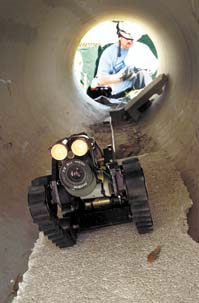
\includegraphics[scale=0.42]{images/search_and_rescue.png}}
		    \only<2>{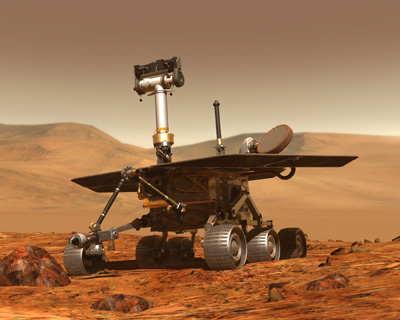
\includegraphics[scale=0.40]{images/mars.png}}
		    \only<3>{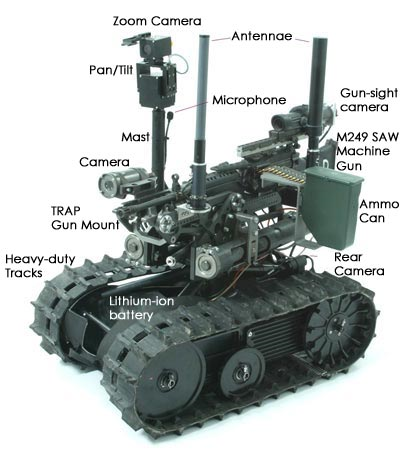
\includegraphics[scale=0.30]{images/army.png}}
    	\end{overprint}
	\end{itemize}
	
\end{frame}
  %\only<4>{



\begin{frame}
\frametitle{Frontier-Based Exploration}
\begin{itemize}
  \item A modern approach to exploration is based on \emph{frontiers}
  \item \emph{Frontier}: separates known regions from unknown regions 
  	\begin{itemize} 
		\item Set of \emph{unknown} points 
		\item Each has at least one \emph{open-space} neighbor
  	\end{itemize} \pause
  \item The robot moves towards a frontier and discover new regions 
  %By moving towards frontiers, robots keep discovering new regions
  \begin{itemize}
  	  \item Yamauchi: first to show a frontier-based strategy
  	  \item \citep{yamauchi_frontier-based_1997,yamauchi_frontier-based_1998}
  	  \item His work preceeded many others 
  	  \item e.g.
  	  \citep{burgard05tro,lau_behavioural_2003,sawhney_fast_2009}%,burgard_collaborative_2000}
  \end{itemize}
\end{itemize}
\end{frame}

\begin{frame}
\frametitle{Problem Definition}
\begin{itemize}
  \item Given: sequence of observations $\langle O_0,\ldots,O_t\rangle$
  \item Observation $O_x$ is a tuple $\langle G_x, P_x, R_x\rangle$
  \begin{itemize}
	  \item $G_x:=$ occupancy-grid of time $x$
	  \item $P_x:=$ robot pose of time $x$
	  \item $R_x:=$ range sensor readings of time $x$
  \end{itemize}
  \item \emph{Frontier Detection Problem}: return all frontiers existing at
  time $t$
\end{itemize}
\end{frame}

\begin{frame}
\begin{figure}
 \centering
 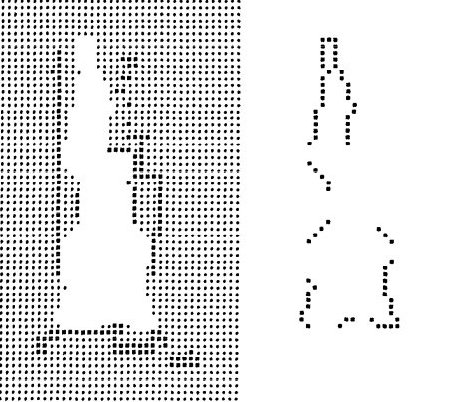
\includegraphics[width=0.6\columnwidth,keepaspectratio]{images/frontiers_example_only_frontiers.jpg}
 \caption{Image taken from \citep{yamauchi_frontier-based_1998}: evidence
 grid, frontier points (from left to right).}
 %, extraction of different frontiers (from left to right).}
\end{figure}
\end{frame}

\begin{frame}
\frametitle{Frontier-Based Exploration Diagram}
\centering
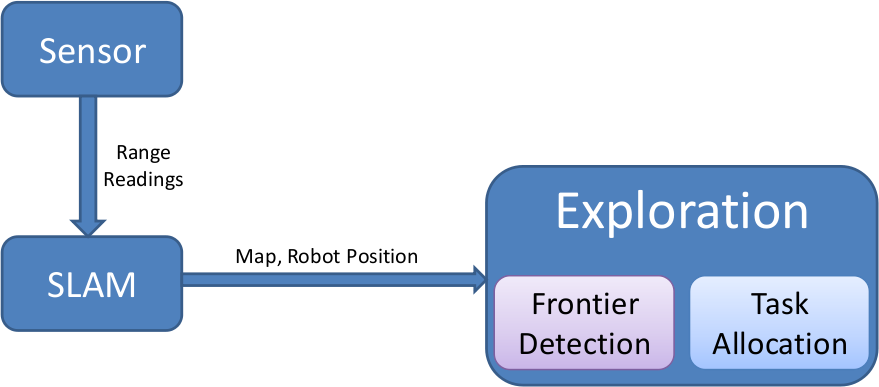
\includegraphics[width=0.8\columnwidth,keepaspectratio]{images/exploration_diagram.png}
\begin{itemize}
  \item Sensor: provides range readings of the environment
  \item SLAM: builds a map of the environment
  \item Exploration: sends robots to chosen targets in the environment 
\end{itemize}
\end{frame}

\begin{frame}
\frametitle{Simulaneous Localization and Mapping}
\begin{itemize}
  \item Builds a map of an unknown environment while navigating
  \item Robots do not utilize any \emph{a priori} knowledge of the environment
  \item \emph{SLAM} is a concept, not an algorithm \pause
  \item Two main approaches:
  \begin{itemize}
    %\item \emph{Extended Kalman Filter} 
    %	\begin{itemize}
	      \item Only one map that is composed from observed landmarks   
	%	\end{itemize} 
	%\item \emph{Particle Filter} 
	 %   \begin{itemize}
		  \item More than one map (possible hypotheses of the world state)
	 %     \item Each particle is a possible hypothesis of the world state
	 %     \item State: set of variables (e.g map of explored area, robot position)
	%	\end{itemize}
  \end{itemize}
\end{itemize}
\end{frame}




\begin{frame}
\frametitle{Outline}
	\begin{itemize}    	    	
	 \item Previous methods for computing frontiers: Slow!
		\begin{itemize}
		 \item searches the entire map with every call
		\end{itemize}
	 \item Two approaches for frontier detection: \WFD, \FFD
	 	\begin{itemize}
		 	\item \WFD: explores only known regions
		 	\item \FFD: explores only border of known regions
		\end{itemize}
	 \item Theoretical analysis (correctness, complexity)
	 \item Incremental versions of \WFD: \WFDINC, \WFDIP
	 \item Results: improvement of 1-2 orders of magnitude over \SOTA
	\end{itemize}
\end{frame}

% \subsection*{Exploration}
% \begin{frame}
% \frametitle{Exploration}
% \begin{itemize}
%   \item Exploring an unknown area is a fundmental problem in robotics
%   \item Gain as much new information as possible within a bounded time
%   \item Efficient exploration methods are used in a variety of applications:\begin{itemize}
%   	  \item Search and Rescue \citep{Kitano99robocuprescue}
%   	  \item Planetary Exploration \citep{apostolopoulos2001robotic}
% 	  \item Military Uses \citep{hougen2000miniature}
%     \end{itemize}
% \end{itemize}
% \end{frame}




\begin{frame}
\frametitle{Existing Frontier Detection is Slow}
\begin{tikzpicture}[remember picture, overlay]
	\node[xshift=-10pt,yshift=-92pt]  at (current page.north east)
	{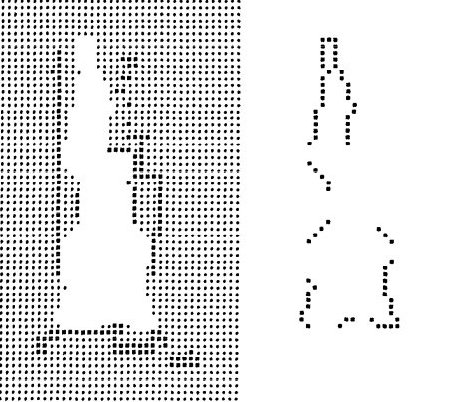
\includegraphics[width=0.25\columnwidth,keepaspectratio]{images/frontiers_example_only_frontiers.jpg}};
\end{tikzpicture}
\begin{itemize}
  \item Traditional algorithms rely on computer vision methods 
  %\item Most frontier detection methods are based on computer vision techniques
  \begin{itemize}
    \item e.g. edge detection and region extraction
  \end{itemize}
  
  \item Process the entire map data with every execution \pause
  \item Map size is larger than typical image size 
  \item Existing frontier detection methods take $\sim$10--30 seconds to run
  	\begin{itemize}
  	  \item Even on powerful computers 
  	  \item Exploring a large area forces the robot to wait in its spot 
  	  %\item Frontier detection is called only when the robot
  	  %arrives at its target 
  	\end{itemize} 
  
  %the algorithm finishes
  
  \pause
%   \item Thus, real-time frontier detection can shorten the exploration time
\end{itemize}
\begin{block}{Result}
	\center Efficient frontier detection can shorten the exploration time
\end{block}
 
\end{frame}

% \begin{frame}
% \frametitle{Single-Robot Example}
% 	\begin{figure}
% 	 \centering
% 	 \includegraphics<+>[width=0.85\columnwidth,keepaspectratio]{images/single_1.JPG}
% 	 \includegraphics<+>[width=0.85\columnwidth,keepaspectratio]{images/single_2.JPG}
% 	 \includegraphics<+>[width=0.85\columnwidth,keepaspectratio]{images/single_3.JPG}
% 	\end{figure}
% \end{frame}

\subsection*{Example}
\begin{frame}
\frametitle{Multi-Robot Example}
	\begin{figure}
	 \centering
	 \includegraphics<+>[width=0.85\columnwidth,keepaspectratio]{images/multi_1.JPG}
	 \includegraphics<+>[width=0.85\columnwidth,keepaspectratio]{images/multi_2.JPG}
	\end{figure}
\end{frame}


% \begin{frame}
% 
% \begin{itemize}
%   \item \emph{SLAM} is a concept, not an algorithm \pause
%   \item \emph{Extended Kalman Filter} 
%     \begin{itemize}
%       \item Only one map that is composed from observed landmarks   
% 	\end{itemize} \pause
%   \item bla 
%     \begin{itemize}
%       \item Each particle is an instance of the system state at a certain time
% 	\end{itemize}
% \end{itemize}
% \end{frame}